\subsection{Demographic factors: \textit{Population, age, urbanisation}}\label{sec:quantification_demographic}

\subsubsection{Definition}

Demographic factors encompass a range of population characteristics, including
age distribution, population growth rates, urbanisation levels, migration
patterns, and household composition. These factors are crucial determinants in
forecasting demand patterns, labour market dynamics, and consumption trends,
which in turn affect supply chains and resource management.

In the context of the scenarios and modelling within FutuRaM, demographic
factors could influence the demand for certain commodities, the availability of
labour for new recycling technologies, and the generation of waste materials.
As populations grow and become more urbanised, the demand for electronics,
energy, and transportation increases, which in turn raises the demand for
critical raw materials necessary for these technologies. Age distributions can
affect the workforce available for the recycling industry and potentially shift
consumption patterns, as older populations might consume differently compared
to younger demographics.


\boxparameter{Demographics}{Current trends}{Current trends}{Current trends}


\subsubsection{Justification for setting as an external scenario factor}

Demographics undoubtedly exert a significant influence on supply and demand
patterns within any resource environment.~\cite{irp2019globalresourcesoutlook} As such, demographic factors play a
role in shaping the demand for CRMs and the efficiency of waste management
systems. However, within the scope of FutuRaM's scenario modelling, these
demographic elements are treated as background variables.

A standard set of demographic projections is applied across all scenarios,
contributing to the baseline assumptions but not serving as the primary driver
of change in the model. By setting demographics as an external factor,
FutuRaM's scenarios can abstract from the nuanced impacts of demographic
changes, allowing for a clearer interpretation of how policy levers directly
affect SRM outcomes.

Furthermore, the structure of FutuRaM's models is designed to be sufficiently
adaptable to account for future demographic shifts. As new data become
available, they can be integrated into the existing models, allowing for
regular updates that keep pace with the evolving demographic landscape. This
flexibility ensures that the model's outputs remain both relevant and grounded
in the most current understanding of demographic factors, while the focus stays
on the core objectives of resource management and the evaluation of policy
efficacy.


\boxreview{Data for other demographic factors such as urbanisation, gender or persons per household can be added here if the waste stream models require it.}

\subsection*{Population projections}

\subsubsection{Sources for demographic data}

The population projections in this report have been produced from the most
recent data provided by Eurostat and the UK Office of National Statistics
(ONS)~\cite{eurostat2023population, ons2023population, vanella2020populationprojections}.

It was decided to `re-model' this data, rather than extract it from the
population figures in the SSP2 baseline scenario
datasets~\cite{ssp2017narrative, samir2017ssp} to which the background of
FutuRaM's scenarios are (broadly) aligned. This allows the use of the most
up-to-date and `raw' data possible.

\autoref{fig:population} shows the normalised population projections for the EU27+3 and the UK. The index is set to 1 for the year 2020.
An interactive figure can be viewed \href{https://futuram-project.github.io/FutuRaM.github.io/WP2/assets.html}{here~\faLink}


\begin{figure}[h!]
      \centering
      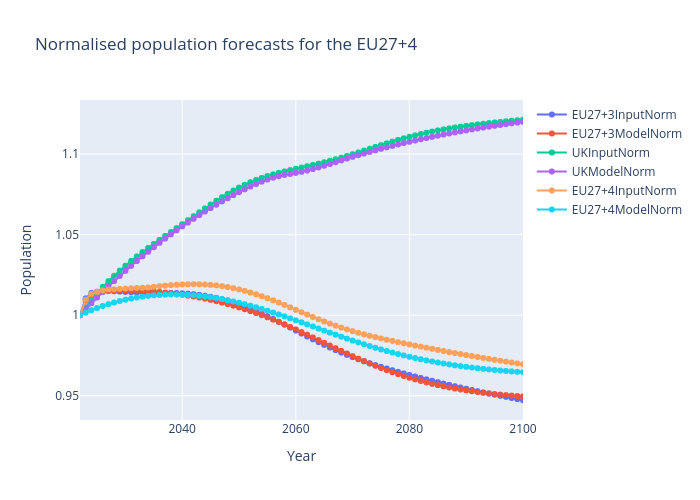
\includegraphics[width=\linewidth]{130quantification/external/population.png}
      \caption{Population projections for the EU27+3 and the UK}\label{fig:population} 
\end{figure}

\subsubsection{EU27 + 4}

\textbf{Data source:}~\cite{eurostat2023population}

\subsubsubsection{Population modelling results:}

The full results of the population modelling are presented in
\autoref{tab:population}.

\subsubsubsection{Highlights:}

\begin{itemize}
      \item The EU population is projected to rise from 446.7 million in 2022, peaking at
            453.3 million in 2026 (+1.5\%), before decreasing to 447.9 million in 2050 and
            further to 419.5 million in 2100.
      \item An increase of 5.8 years is expected in the median age of the EU population
            between 2022 and 2100.
      \item By 2100, the number of individuals aged 80 and over in the EU is projected to
            reach 64.0 million.
\end{itemize}

Populations evolve over time due to demographic factors: births, deaths, and
migration. Each of these factors influences the population's structure.
Presently, the EU is experiencing a trend of ageing in its population due to
the prevailing levels of fertility and mortality.

EUROPOP2023 offers deterministic projections based on `what-if' scenarios.
These scenarios are formed on anticipated courses for fertility, mortality, and
migration. A partial convergence is assumed among the countries in the
EUROPOP2023 projection concerning fertility, mortality, and migration patterns.
The methodology employed is primarily based on past projection exercises.
Furthermore, this study accounts for the impact of the COVID-19 pandemic and
the mass influx due to the conflict between Russia and Ukraine.

It is projected by Eurostat that all EU Member States and the three EFTA
countries will experience continued population ageing. The population in 2100
is predicted to be lower than in 2022, with a decline in the working-age
demographic. There's an observed trend of ageing within the elderly demographic
itself. Migration can both alleviate and accelerate the ageing process. It
depends on whether there's an influx or outflow of the working-age population.
For instance, the search for better job opportunities can lead to a
considerable outflow. Consequently, age dependency ratios are set to rise,
posing challenges for public expenditure on pensions, healthcare, and long-term
care.

\subsubsubsection{Method}

Eurostat provides international projections for the European Union (EU) and the
European Free Trade Association countries, which include Iceland,
Liechtenstein, Norway, and Switzerland. Unlike the UN's projections, Eurostat's
are deterministic in nature. Their most recent projection, dating from 2020,
presents a base variant along with four other variants, starting with the
baseline year 2019. In the base variant, it is forecasted that the EU-27
population will decline by nearly 7 percent or about 30 million people by 2100.
However, in the medium term, the population is expected to grow until 2025,
reaching about 449 million people, before reducing to 416 million by 2100.
Country-specific, sex, and age data are available in Eurostat`s database.

The final projection starts with the 2022 population divided by sex and age.
Mortality rates are applied to determine the number of deaths. Numbers for
non-EU and EU immigrants are computed. For the years 2022 and 2023, refugees
under TP are also included. Emigrants, including refugees under TP for the
years 2024 to 3033, are then subtracted. Based on this, the end-of-year
population and the working-age population are computed. Using these figures,
additional non-EU immigrants are calculated, and the end-of-year population is
re-assessed. This allows for the computation of live births, total deaths,
immigration, and emigration for 2022.

\subsubsubsection{Scenarios}

Eurostat also considers five alternative scenarios besides the baseline for
EUROPOP2023. These are: lower fertility, lower mortality, zero net migration,
decreased non-EU immigration, and increased non-EU immigration. For instance,
the lower fertility scenario posits a total fertility rate that's 20\% less
than the baseline for each projection year (2023 -- 2100). This implies fewer
live births yearly compared to the baseline. The lower mortality scenario
suggests a life expectancy at birth in 2100 that's two years more than the
baseline. Migration scenarios include zero net migration, 33\% less non-EU
immigration each year, and 33\% more non-EU immigration every year throughout
the projection horizon.

\subsubsection{UK}

\textbf{Data source:}~\cite{ons2023population}


\begin{itemize}
      \item New data will be released January 2024.
      \item No scenarios were developed due to the additional uncertainty in the underlying
            data related to the CoViD-19 pandemic-related fluctuations.
\end{itemize}

\subsubsubsection{Population modelling results:}

The full results of the population modelling are presented in
\autoref{tab:population}.

\subsubsubsection{Population Projections}

The UK population in mid-2020 was estimated at 67.1 million. Over the decade to
mid-2030, it's projected to rise by 2.1 million (3.2\% increase), in comparison
to a 6.9\% increase between 2010 and 2020. Over the next 25 years, the
projected growth is 3.9 million (5.8\%), less than the 15.6\% growth between
mid-1995 and mid-2020.

In contrast to the EU27+3, the UK population is projected to continue to
continue growing (slowly) until 2100, the end of the projection period, when it
reaches 76 million.

\subsubsubsection{Assumptions:}
\begin{itemize}
      \item Long-term averages are based on a 22-year period, excluding the 1990s.
      \item Long-term average falls within the ranges given by expert advisory feedback.
      \item Estimated international migration data is used for the years ending mid-2021
            and mid-2022.
      \item Linear interpolation is used from mid-2022 up to mid-2026.
      \item A three-year average of data from mid-2020 to mid-2022 is used for starting the
            linear interpolation for mid-2022.
      \item UK completed family size to reach 1.59 children per woman by 2045.
      \item Annual improvement in UK mortality rates will be 1.2\% for most ages by 2045.
      \item Net international migration to the UK will average +205,000 from mid-2027
            onwards.
\end{itemize}

\subsubsubsection{Methodology}
Projections are produced for successive years from one mid-year to the next. Age-based calculations are made to account for net migration, deaths, and births. Details such as migration timing, death rates, birth rates, and the ratio of male-to-female births are factored into the calculations. Projections are made for each UK country and then aggregated for broader regions.

\subsubsubsection{Strengths and Limitations}
Projections are based on the latest available data but are not forecasts. The inherent uncertainty in the data and the unpredictability of future events means projections may not align with future outcomes. Factors like political and economic changes can also impact population growth, and events like the UK leaving the EU or the COVID-19 pandemic are not explicitly factored in. While this bulletin focuses on projections up to mid-2045, the data includes projections up to mid-2120, which have greater inherent uncertainty.

\subsubsubsection{Merging the EU27+3 and the UK into a unified population model}

As the world undergoes the demographic transition, the relevance of Verhulst's
logistic model has resurged, providing an adequate representation of current
population growth trends. This logistic population growth dynamic is critical
for achieving global sustainable development.

These projections are informed by the finite reserves of primary exhaustible
resources and the ongoing trend of declining birth rates. These indications
suggest a shift towards a new equilibrium state for the planet that aligns with
heightened industrial and technological capacities and improved healthcare
standards. By constructing logistic models that depict the growth dynamics of
the global population and individual continents, we can forecast population
sizes and their growth rates for the next two centuries. The insights garnered
present opportunities for the regulation and optimal management of global
demographic resources.

\subsubsection{Projection Methodology}

\textbf{Methodology source:}~\cite{vanella2020populationprojections}

Population projections underpin many political and economic decisions at
various levels. Often, the users lack the expertise to fully grasp the methods
and limitations of the projections they rely on.

Population development is contingent upon three primary factors: fertility, net
migration, and mortality. Usually, a projection starts with the age- and
sex-specific numbers at a given time. Using estimates for the future
development of the three determinants, the population is projected forward.
Forecasts often refine mortality and migration by age and sex.

Projection methodologies fall into deterministic and stochastic categories.
Deterministic models, being the most widespread, set parameters in one or more
scenarios. Their strengths lie in ease of use, adaptability to changes in
parameters, and straightforwardness for non-experts. A prominent deterministic
method is the cohort component method (CCM) which separately simulates
fertility, migration, and mortality before integrating them into a projection.
Given a population \(P_{t-1}\) at the end of period \(t-1\), the CCM updates
this using births \(B_t\), net migration \(M_t\), and deaths \(D_t\) as:

\[ P_t = P_{t-1} + B_t + M_t - D_t \]

However, deterministic models face challenges. They:
\begin{itemize}
      \item Overlook the probabilistic nature of population processes.
      \item Rely on rigid future assumptions with low individual probabilities of
            occurrence.
      \item Limit the number of considered scenarios, inadequately reflecting future risk.
      \item Lack probabilistic quantification for identified futures.
      \item May be biased by experts' subjective assessments.
\end{itemize}

In contrast, stochastic models view parameters as random variables. While
deterministic models might assume fixed values for determinants like \(G_t,
M_t\), and \(S_t\) in certain scenarios, stochastic models see these as
probabilistic, represented as:

\[ \tilde{B}_t = \tilde{B}_{t-1} + \tilde{G}_t + \tilde{M}_t - \tilde{S}_t \]

Yet, it's essential to understand that no forecast offers absolute truth. Their
aim isn't predicting unexpected events, but extrapolating core demographic
trends. Both deterministic and stochastic methods exist to quantify forecast
uncertainty.

Applying these results in real-world scenarios warrants a cautious approach.
Past trends might not persist in the future. For instance, population growth
isn't just about demographics but also infrastructure. Can a housing market
accommodate growth? Will cities meet their limits? Projections inherently carry
assumptions. For instance, regions must meet housing demands, and urban
challenges arise from positive population growth, such as the need for expanded
childcare or public transport infrastructure.

Predicting and managing future global population growth stands as a paramount
challenge for humanity. Most contemporary researchers believe there's a ceiling
to the planet's `carrying capacity'. Come 2022, Earth's population is
anticipated to hit the eight billion mark. UN predictions suggest that by 2100,
this number will rise to ten billion. However, there's an observable trend
towards smaller family sizes, with birth rates currently hovering around the
replacement rate of 2.1 children per woman. Should global fertility rates align
with family replacement levels (2.0) by 2100, Earth's population is projected
to stabilise between ten and eleven billion. The emergence of new statistical
data necessitates updates to global population growth models. Where once the
Verhulst logistic model was deemed inadequate for characterising global
population growth dynamics, the tapering growth rate now reaffirms its
applicability. Many recent studies have leveraged the logistic growth model.
Our analyses confirm that Earth's population growth rate aligns closely with a
quadratic function, mirroring the Verhulst equation (Fig. 4). All subsequent
computations will employ the Verhulst logistic model:

\begin{equation}
      \frac{dY}{dt} = a \cdot Y - b \cdot Y^2
\end{equation}

The solution to equation (8) will be sought as a logistic function:

\begin{equation}
      Y = g + \frac{b}{1 + A \exp(-a(t - t_0))}
\end{equation}

Function \( Y(t) \) parameters were ascertained using the least squares method,
ensuring maximal alignment between the function's value and the existing
statistical data. The parameter \( g \) was presumed equal to the initial
population size at the start of observations (\( t_0 =1900 \)).

\subsubsubsection{Curve Fitting Explanation}

Terms with subscript 1 describe the initial logistic component, charting
population growth from 2022 to 2042.

Subscript 2 terms Correspond to the second logistic component, which outlines
post-2042 population decline.

\begin{description}[style=nextline, leftmargin=2cm]
      \item[\(\mathbf{b_1}\)] 
            Represents the initial population at the start of the observation period - Europe's population in 1900 per the model's parameters.

      \item[\(\mathbf{b_1}\)] 
            Denotes the carrying capacity of population growth, effectively indicating the population apex achievable via the first logistic function.

      \item[\(\mathbf{A_1}\)] 
            Influences the gradient of the first growth phase. Higher values result in steeper population inclines.

      \item[\(\mathbf{a_1}\)] 
            Represents the growth rate of the initial logistic function, dictating how swiftly the population nears the carrying capacity \( b_1 \).

      \item[\(\mathbf{t_1}\)] 
            Marks the inflection point in the first logistic phase, signifying the period of maximum growth velocity.

      \item[\(\mathbf{b_2}\)] 
            Illustrates the decline's carrying capacity, indicating the population decrease as projected by the second logistic function.

      \item[\(\mathbf{A_2}\)] 
            Determines the gradient of the decline phase, with larger values resulting in sharper declines.

      \item[\(\mathbf{a_2}\)] 
            Represents the rate of decline in the latter logistic function, determining the speed at which the population reaches the decline's carrying capacity \( b_2 \).

      \item[\(\mathbf{t_2}\)] 
            Highlights the inflection point during the decline phase, marking the period where the decrease is most rapid.
\end{description}


\begin{table}[h!]
      \centering
      \small
      \caption{Population projections for the EU27+4}\label{tab:population}
      \begin{tabular}{|C{1.5cm}|C{1.5cm}|C{1.5cm}|C{1.5cm}|C{1.5cm}|}
            \hline
            \rowcolor{headerblue} % Applying the header color
            \textcolor{white}{\textbf{YEAR}} & \textcolor{white}{\textbf{MEDIAN AGE}} & \textcolor{white}{\textbf{EU27+4} (million)} & \textcolor{white}{\textbf{EU27+3} (million)} & \textcolor{white}{\textbf{UK} (million)} \\
            \hline
            \csvreader{csvs/population.csv}{}{\csvcoli& \csvcolii& \csvcoliii& \csvcoliv& \csvcolv\\ \hline}
      \end{tabular}

\end{table}



\clearpage
\subsubsection{Incorporation of demographic factors into individual waste stream models}


\boxws{This section will be filled out with the details of exactly how the demographic parameters are incorporated into your stock and flow models}


\wasteSubsubsubsecBATT
\begin{itemize}
    \item X
\end{itemize}

\wasteSubsubsubsecCDW
\begin{itemize}
    \item X
\end{itemize}

\wasteSubsubsubsecELV
\begin{itemize}
    \item X
\end{itemize}

\wasteSubsubsubsecMIN
\begin{itemize}
    \item X
\end{itemize}

\wasteSubsubsubsecSLASH
\begin{itemize}
    \item X
\end{itemize}

\wasteSubsubsubsecWEEE
\begin{itemize}
    \item X
\end{itemize}


\subsubsection{Conclusion}


\boxreview{This conclusion will be compiled once the individual waste stream sections for each parameter are complete.}


\sectionEndlines
\clearpage
